\documentclass[conference]{IEEEtran}
\IEEEoverridecommandlockouts
% The preceding line is only needed to identify funding in the first footnote. If that is unneeded, please comment it out.
\usepackage{cite}
\usepackage{amsmath,amssymb,amsfonts}
\usepackage{algorithmic}
\usepackage{graphicx}
\usepackage{textcomp}
\usepackage{xcolor}
\def\BibTeX{{\rm B\kern-.05em{\sc i\kern-.025em b}\kern-.08em
    T\kern-.1667em\lower.7ex\hbox{E}\kern-.125emX}}
\begin{document}

\title{CENG435 Term Project Part 1
}

\author{\IEEEauthorblockN{Ahmet Kürşad Şaşmaz}
\and
\IEEEauthorblockN{Ali Şen}
}

\maketitle

\section{Introduction}
In this CENG435 Term Project, participants worked on an already designed network topology. Shortest path from source to destination was found by calculating the average RTT values between every node. After, topology was reset according to shortest path. Finally, end to end delay was tested with respect to network emulation delay.

\section{Set Up The Environment}
\subsection{Network Topology}
There was 5 nodes on the topology. Names of the nodes were \textbf{s},\textbf{r1},\textbf{r2},\textbf{r3},\textbf{d}.
Connection link table is given below.
\begin{table}[h]
\centering
\begin{tabular}{|l|l|}
\hline
\textbf{s}  & \textbf{r1} \\ \hline
\textbf{s}  & \textbf{r2} \\ \hline
\textbf{s}  & \textbf{r3} \\ \hline
\textbf{d}  & \textbf{r1} \\ \hline
\textbf{d}  & \textbf{r2} \\ \hline
\textbf{d}  & \textbf{r3} \\ \hline
\textbf{r1} & \textbf{r2} \\ \hline
\textbf{r3} & \textbf{r2} \\ \hline
\end{tabular}
\end{table}

\subsection{Initial Configure Scripts}

Initial configure scripts were for node \textbf{r1} and node \textbf{r2}. Before the server up, configure scripts were run on related nodes.

\subsection{Server/Client Files}

Every node had capability to behave server and client at the same time. In order to provide this, threading paradigm was used. Every node had different purposes.
\subsubsection{\textbf{s}}
\begin{itemize}
    \item Get data from \textbf{r1} and send back.
    \item Get data from \textbf{r2} and send back.
    \item Get data from \textbf{r3} and send back.
\end{itemize}
\subsubsection{\textbf{r1}}
\begin{itemize}
    \item Get data from \textbf{r2} and send back to \textbf{r2} and send copies of data to \textbf{s} and \textbf{d}, and keep a log of data and send time.
    \item Get data from \textbf{s} and keep a log of data and receive time.
    \item Get data from \textbf{d} and keep a log of data and receive time.
\end{itemize}
\subsubsection{\textbf{r2}}
\begin{itemize}
    \item Create data packets and send it to \textbf{s}, \textbf{d}, \textbf{r1}, \textbf{r3}, and keep a log of data and send time. 
    \item Get data from \textbf{s} and keep a log of data and receive time.
    \item Get data from \textbf{d} and keep a log of data and receive time.
    \item Get data from \textbf{r1} and keep a log of data and receive time.
    \item Get data from \textbf{r3} and keep a log of data and receive time.
\end{itemize}
\subsubsection{\textbf{r3}}
\begin{itemize}
    \item Get data from \textbf{r2} and send back to \textbf{r2} and send copies of data to \textbf{s} and \textbf{d}, and keep a log of data and send time.
    \item Get data from \textbf{s} and keep a log of data and receive time.
    \item Get data from \textbf{d} and keep a log of data and receive time.
\end{itemize}
\subsubsection{\textbf{d}}
\begin{itemize}
    \item Get data from \textbf{r1} and send back.
    \item Get data from \textbf{r2} and send back.
    \item Get data from \textbf{r3} and send back.
\end{itemize}

\subsection{Synchronization of Server Times}

In order to get the time packet send and packet receive time correctly, the servers had to be synchronized with respect to time. To provide this; \\
\textbf{sudo ntpdate -qu north-america.pool.ntp.org} \\
command was executed in every node.

\section{Discovering The Network Topology}


\subsection{Starting The Servers}

Because \textbf{s} and \textbf{d} were mirroring nodes, these were initialized first. \\
Then \textbf{r1} and \textbf{r3} were initialized. \\
Because \textbf{r2} was data initializer node, \textbf{r2} was initialized last.\\
Totally, 1000 packets were used for every link.

\subsection{Collecting The RTT Values}

Logs were brought together to be compared. About one third of packets were lost. Matched data packets were sorted out, and average of the difference between receive time and send time was calculated for every link. The table of average RTT value of links is below.
\begin{table}[h]
\centering
\begin{tabular}{|l|l|l|}
\hline
\textbf{s}  & \textbf{r1} & 100.3ms \\ \hline
\textbf{s}  & \textbf{r2} & 104.6ms \\ \hline
\textbf{s}  & \textbf{r3} & 0.5ms   \\ \hline
\textbf{d}  & \textbf{r1} & 85.4ms  \\ \hline
\textbf{d}  & \textbf{r2} & 102.8ms \\ \hline
\textbf{d}  & \textbf{r3} & 0.5ms   \\ \hline
\textbf{r1} & \textbf{r2} & 258.0ms \\ \hline
\textbf{r3} & \textbf{r2} & 224.5ms \\ \hline
\end{tabular}
\end{table}

\subsection{Finding The Shortest Path}

\begin{itemize}
    \item nodeSet = \{\}
    \item s = 0
    \item d = inf
    \item r1 = inf
    \item r2 = inf
    \item r3 = inf
    \item nodeSet = \{s\}
    \item r1 = 100.3
    \item r2 = 104.6
    \item r3 = 0.5
    \item nodeSet = \{s,r3\}
    \item d = 0.5
    \item nodeSet = \{s,r3,d\}
    \item nodeSet = \{s,r3,d,r1\}
    \item nodeSet = \{s,r3,d,r1,r2\}
\end{itemize}

Shortest path table is below.

\begin{table}[h]
\centering
\begin{tabular}{|l|l|}
\hline
\textbf{s}  & \textbf{r1} \\ \hline
\textbf{s}  & \textbf{r2} \\ \hline
\textbf{s}  & \textbf{r3} \\ \hline
\textbf{r3} & \textbf{d}  \\ \hline
\end{tabular}
\end{table}

\section{Reset The Environment}
\subsection{Network Topology}
There was 5 nodes on the topology. Names of the nodes were \textbf{s},\textbf{r1},\textbf{r2},\textbf{r3},\textbf{d}.
Connection link table is given below.
\begin{table}[h]
\centering
\begin{tabular}{|l|l|}
\hline
\textbf{s}  & \textbf{r1} \\ \hline
\textbf{s}  & \textbf{r2} \\ \hline
\textbf{s}  & \textbf{r3} \\ \hline
\textbf{r3} & \textbf{d} \\ \hline
\end{tabular}
\end{table}

\subsection{Configure Scripts}

Because there were 3 different experiments, 3 different configuration files for every link between the nodes \textbf{s}, \textbf{r3} and \textbf{d}. To configure the links, two different configuration scripts were prepared for \textbf{s} and \textbf{r3}. Before the server up for specific experiment, configure scripts for related experiment were run on related nodes.

\begin{table}[h]
\centering
\begin{tabular}{|l|l|l|}
\hline
Experiment & Network Emulation Delay & Jitter \\ \hline
1          & 20ms                    & 5ms    \\ \hline
2          & 40ms                    & 5ms    \\ \hline
3          & 50ms                    & 5ms    \\ \hline
\end{tabular}
\end{table}

\subsection{Server/Client Files}

Because the shortest path was \textbf{s}-\textbf{r3}-\textbf{d}. Purposes of the nodes were changed.
\subsubsection{\textbf{s}}
\begin{itemize}
    \item Create data packets and send it to \textbf{r3}, and keep a log of data and send time. 
\end{itemize}
\subsubsection{\textbf{r3}}
\begin{itemize}
    \item Get data from \textbf{s} and send it to \textbf{d}.
\end{itemize}
\subsubsection{\textbf{d}}
\begin{itemize}
    \item Get data from \textbf{r3}, and keep a log of data and receive time. 
\end{itemize}

\section{Experiments}

\subsection{Starting The Servers}

For every specific experiment, below were done.
Because \textbf{d} was listening node, it was initialized first. \\
Then \textbf{r3} was initialized. \\
Because \textbf{s} was data initializer node, \textbf{s} was initialized last. \\
Totally, 3000 packets were sent, and send time and receive time were recorded by \textbf{s} and \textbf{d} \\
Finally, the scripts were terminated.

\subsection{Collecting The End to End Delay Values}

Logs were brought together to be compared. About one sixth of packets were lost. Matched data packets were sorted out, differences of the receive time and the send time were calculated for every experiment, and plotted on a graph with \% 95 confidence interval by using Excel.

\begin{figure}[h]
  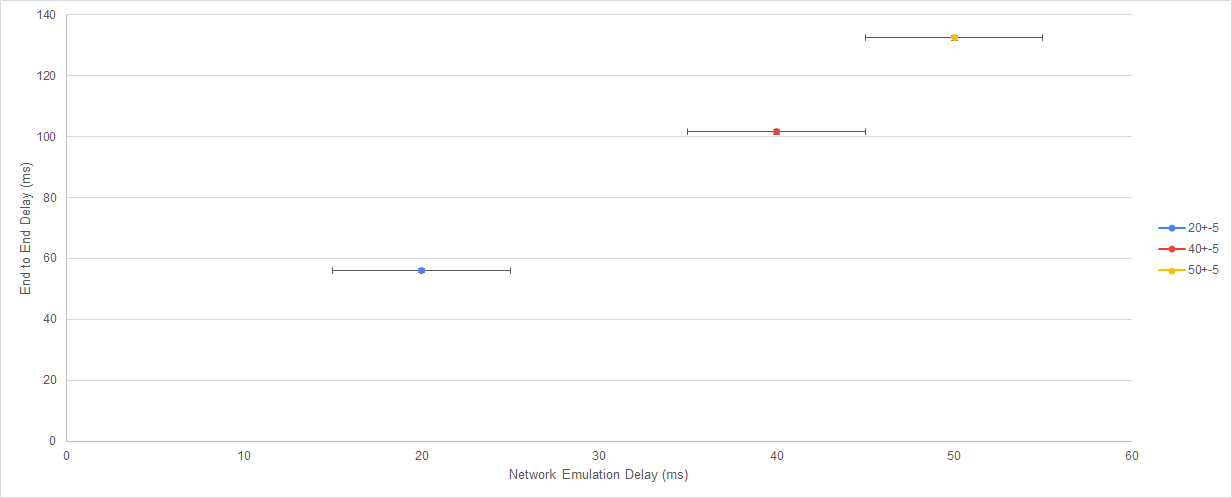
\includegraphics[width=\linewidth]{plot_stat.png}
  \caption{Network Emulation Delay vs End to End Delay}
  \label{fig:plot}
\end{figure}

Figure \ref{fig:plot} Network Emulation Delay vs End to End Delay.

\begin{table}[h]
\centering
\begin{tabular}{|l|l|l|l|}
\hline
Network Emulation Delay & $\mu$ & $\sigma$ & Error \\ \hline
20ms $\pm$ 5ms              & 56ms  & 19ms     & 1ms     \\ \hline
40ms $\pm$ 5ms              & 102ms & 21ms     & 1ms     \\ \hline
50ms $\pm$ 5ms              & 132ms & 19ms     & 1ms     \\ \hline
\end{tabular}
\end{table}

According to the graph, as network emulation delay between the links increases, end to end delay from source to destination increases almost linearly. When $d$ stands for network emulation delay and $p$ stands for total processing time of nodes, theoretical end to end delay formula becomes $2d \pm 5ms + p$. According to this formula, when network emulation delay increases, end to and delay increases twice. It can be seen that the results of the experiments were consistent with the theoretical calculations.

\section{Discussions}
In real life, most of the links are used by many users most of the time packets affected by the delay but in our topology nobody our link except us because we create the servers and clients and they are under control of us. That is why there would be no delay or the same delays for other router unless we configure the routers. This means that all packets would give the same amount of delay. It doesn't matter which router our packets pass through, to prevent this we configure them. The advantage of packet switching is sending and receiving data at the same time when the link is being used. But on the other hand, we observe some packet loss which we didn't want in real life and that is the disadvantage of such a topology.

\end{document}
